%%%%%%%%%%%%%%%%%%%% author.tex %%%%%%%%%%%%%%%%%%%%%%%%%%%%%%%%%%%
%
% sample root file for your "contribution" to a contributed volume
%
% Use this file as a template for your own input.
%
%%%%%%%%%%%%%%%% Springer %%%%%%%%%%%%%%%%%%%%%%%%%%%%%%%%%%


% RECOMMENDED %%%%%%%%%%%%%%%%%%%%%%%%%%%%%%%%%%%%%%%%%%%%%%%%%%%
\documentclass[graybox]{svmult}

% choose options for [] as required from the list
% in the Reference Guide

\usepackage{mathptmx}       % selects Times Roman as basic font
\usepackage{helvet}         % selects Helvetica as sans-serif font
\usepackage{courier}        % selects Courier as typewriter font
\usepackage{type1cm}        % activate if the above 3 fonts are
                            % not available on your system
%
\usepackage{makeidx}         % allows index generation
\usepackage{graphicx}        % standard LaTeX graphics tool
                             % when including figure files
\usepackage{multicol}        % used for the two-column index
\usepackage[bottom]{footmisc}% places footnotes at page bottom

\usepackage{amsmath}
\usepackage{threeparttable}

\usepackage{booktabs} 

\usepackage{natbib}

% see the list of further useful packages
% in the Reference Guide

\makeindex             % used for the subject index
                       % please use the style svind.ist with
                       % your makeindex program

%%%%%%%%%%%%%%%%%%%%%%%%%%%%%%%%%%%%%%%%%%%%%%%%%%%%%%%%%%%%%%%%%%%%%%%%%%%%%%%%%%%%%%%%%

\begin{document}

\title*{ECG Annotation and Diagnosis Classification Techniques}
% Use \titlerunning{Short Title} for an abbreviated version of
% your contribution title if the original one is too long
\author{Yan Yan, Yige Wu, Xinbing Qin, Lei Wang}
% Use \authorrunning{Short Title} for an abbreviated version of
% your contribution title if the original one is too long
\institute{Yan Yan \at Yan, Shenzhen Institutes of Advanced Technology, Chinese Academy of Sciences, \email{yan.yan@siat.ac.cn}
\and Yige Wu \at Yige, Shenzhen Institutes of Advanced Technology, Chinese Academy of Sciences, \email{yg.wu@siat.ac.cn}
\and Xinbing Qin \at XinBing, Shenzhen Institutes of Advanced Technology, Chinese Academy of Sciences, \email{xb.qin@siat.ac.cn}
\and Lei Wang \at Lei, Shenzhen Institutes of Advanced Technology, Chinese Academy of Sciences, \email{wang.lei@siat.ac.cn}
}
%
% Use the package "url.sty" to avoid
% problems with special characters
% used in your e-mail or web address
%


%%%%%%%%%%%%%%%%%%%%%%%%%%%%%%%%%%%%%%%%%%%%%%%%%%%%%%%%%%%%%%%%%%%%%%%%%%%%%%%%%%%%%%%%% 
% The abstract section


\maketitle
\abstract{ECG annotation had been studied for decades as the development in signal processing and artificial intelligence methods in computer science. In this chapter the typical technique roadmaps of ECG beat annotation (classification) are reviewed. The deep autoencoder neuro network method were introduce after the mention of supervised and unsupervised learning methods as well as the deep belief networks. A preliminary study on deep learning application in ECG classification had been proposed in this chapter, which lead to better results and have great potential both in performance improvement and unlabelled dataset applications.}


%%%%%%%%%%%%%%%%%%%%%%%%%%%%%%%%%%%%%%%%%%%%%%%%%%%%%%%%%%%%%%%%%%%%%%%%%%%%%%%%%%%%%
%%Background
%%%

\section{Background}
The heart is comprised of myocardium which rhythmically contract and thus drive the circulation of blood throughout the human body.
A wave of electrical current passes through the entire heart, which triggers myocardial contraction \citep{clifford2006advanced}.
Electrical propagation spreads over the whole heart in a coordinated pattern generate changes on the body surface potentials which can be measured and illustrated as an electrocardiogram (ECG, or sometimes EKG).
Metabolic abnormalities (a lack of oxygen, or ischemia etc.) and pathological changes of the heart engender variety of ECG, consequently ECG analysis has been a routine part of any complete medical evaluation or healthcare applications.

Automated ECG analysis provides indispensable assist in clinical monitoring, a large number of approaches have been proposed for the task, basically the diagnosis of arrhythmic and further the inspection of heart rate variability or heart turbulence analysis \citep{mar2011optimization}. 
Lots of  ECG annotation and diagnosis classification techniques had been proposed in industrial circles and academic communities. 
As the general steps in a classification problem in a machine learning task, the ECG classification includes data collection, preprocessing, feature extraction, and classification with a classifier. 

Most of literatures described models which were combined by different classifier with features extracted by different feature extraction algorithms.
The ECG classification methods develops at the same pace with the development of classification theories in machine learning and pattern recognition. 
Because of the particularity in medical data collection and data annotation, the developments in ECG classification and detection were not as flourishing as the similar research topics like speech recognition, natural language processing and image processing etc.

In this chapter, we first introduce the basic elements and procedures in a typical ECG classification task, then we would review shortly about the proposed literatures of ECG classification, in the end we would introduce new methods in unsupervised learning for ECG classification. 

%%%%%%%%%%%%%%%%%%%%%%%%%%%%%%%%%%%%%%%%%%%%%%%%%%%%%%%%%%%%%%%%%%%%%%%%%%%%%%%%%%%%%%%%%Technology Roadmap

\section{Technology Roadmap}
ECG classification methods had been developed for decades. With the development of theories in machine learning and data mining, lots of algorithms had been adopted in this domain. Before the review about the methods, it is quite necessary to mention about the common experiment settings and data sets, as well as the framework of a classification problem which illustrated in Figure \ref{fig:1}.


%%%%%%%%%%%%%%%%%%%%%%%%%%%%%%%Fig1%%%%%%%%%%%%%%%%%%%%%%%%%%%%%%%%%%%%%%%%
\begin{figure}[]
\sidecaption
% Use the relevant command for your figure-insertion program
% to insert the figure file.
% For example, with the graphicx style use
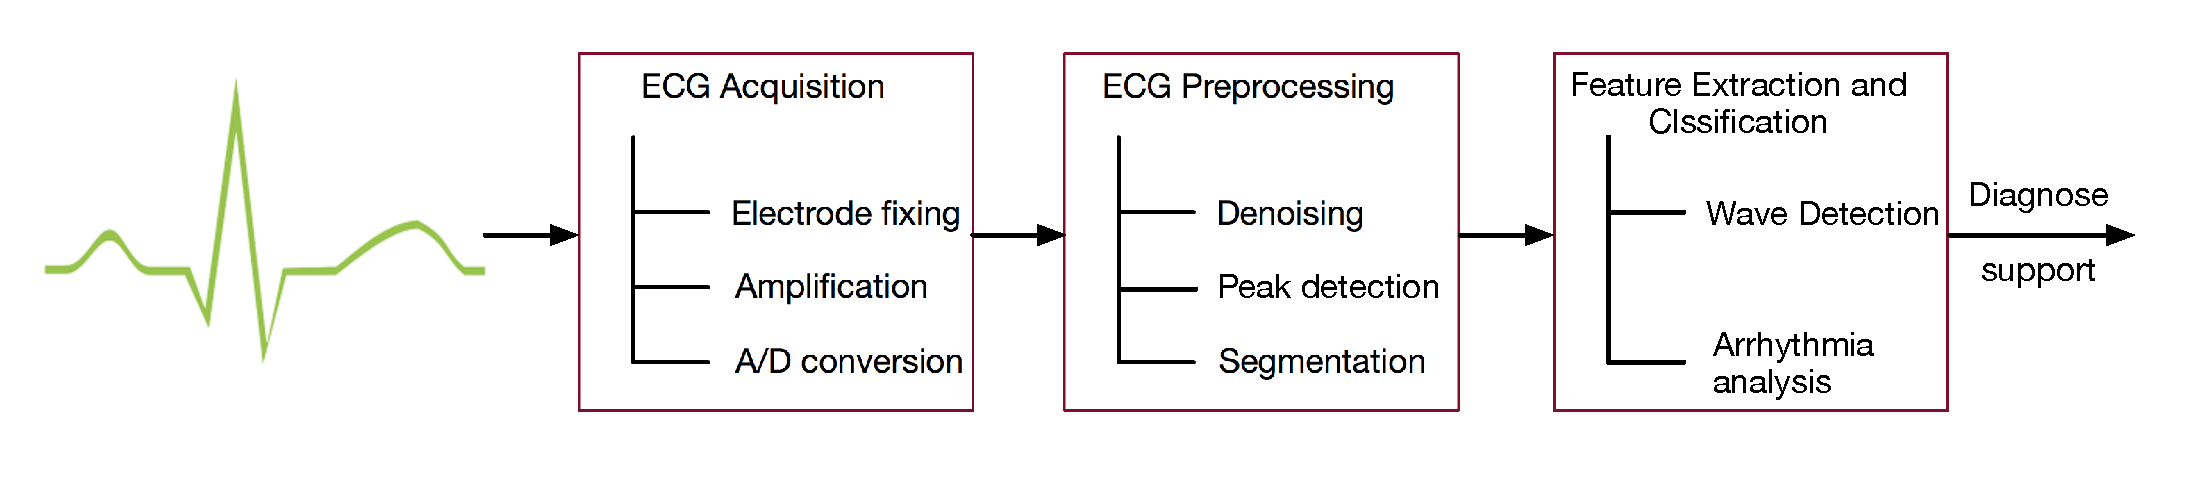
\includegraphics[scale=.32]{classification}
%
% If no graphics program available, insert a blank space i.e. use
%\picplace{5cm}{2cm} % Give the correct figure height and width in cm
%
\caption{The technology roadmap of an ECG classification task.}
\label{fig:1}       % Give a unique label
\end{figure}
%%%%%%%%%%%%%%%%%%%%%%%%%%%%%%%%%%%%%%%%%%%%%%%%%%%%%%%%%%%%%%%%%%%%%%%%%%

\subsection{ECG Acquisition}
Acquiring and storing ECG data were the base for a analyzing task. Errors might be creep into an analysis at any possible stage, thus not only the hardware acquisition system, but also the transmission and storage should be carefully designed. The explantation for the acquisition field could be found in \citep{clifford2006web}. A raw data acquisition task related the digital signal processing and hardware design knowledges are out of the scope in this chapter, a typical ECG signal acquisition process was illustrated in \citep{silva2011dsp}. 

As for the signal acquiring process, different kinds of sample rates might be involved, for common ECG acquisition device the sample rate would be $128Hz$, $250Hz$, $340Hz$ or $500Hz$ even higher. In murine studies, a sampling rate of $2kHz$ is considered sufficiently high \citep{ai1996studies}. Arbitrary resizing would be an ideal procedure to handle with the different sampling rate from different data source to build the datasets for analysis.

\subsection{ECG Signal Preprocessing}
Before the segmentation and feature extraction process, the ECG signals were preprocessed. As in the procedure of collecting ECG signals,  in addition to the ECG signals, the baseline wander (caused by Perspiration, respiration and body movements), power line interference and muscle noise were recorded as well, which had been described in lots of literatures \citep{blanco2008ecg}.
When the filtering methods were proposed and adopted in the preprocessing, the desired information should not be altered. The ECG typically exhibits persistent features like P-QRS-T morphology and average RR interval,  and non-stationary features like individual RR and QT intervals, long-term heart rate trends \citep{clifford2006advanced}. Possible distortions caused by filtering should be quantified in these features.

The filtered ECG signals then were segmented into individual heartbeat waveforms depends on the detected R peaks in a classification task.  The ECG segmentation can be seen as the decoding procedure of an observation sequence in terms of beat waveforms \citep{andreao2006ecg}. Dynamic time warping \citep{vullings1998automated}, time warping \citep{vullings1997ecg}, Bayesian framework \citep{sayadi2009model}, hidden Markov models\citep{andreao2006ecg}, weighted diagnostic distortion \citep{zigel2000weighted}, morphology and heartbeat interval based methods \citep{de2004automatic} and genetic methods \citep{gacek2003genetic} had been used in this sub-task. The state accuracies were close to $100\%$, which would be accurate enough in most online and offline applications. 


\subsection{ECG Feature Extraction and Classification}
After the segmentation for the ECG records, we got plenty of ECG waveform samples with variety categories. Since different physiological disorder may reflect on different type of abnormal heartbeat rhythms. For the task of classification, it is quite important to determine the classes which would be used. In the early literatures, there were no unified class labels for an ECG classification problem. As in the open database MIT-BIH arrhythmia database annotations \citep{mark1982annotated, moody1990bih}, the class label system was build with five beat classes recommended by ANSI/AAMI EC57:1998 standard, i.e., normal beat, ventricular ectopic beat (VEB), supraventricular ectopic beat (SVEB), fusion of a normal and a VEB, or unknown beat type were used in most literature on the classification problems instead of early diversity sub class labels, which could be appropriate in the task since the widely acceptance. 


%%%%%%%%%%%%%%%%%%%%%%%%%%%%%%%%%%%%%%%%%%%%%%%%%%%%%%%%%%%%%%%%%%%%%%%%%%%%%%%%%%%%%%%%%Review on supervised learning
\section{Supervised and Unsupervised Learning Methods in ECG classification}

The application of supervised learning methods had been widely used in ECG for the recognition and classification of different arrhythmia types.
Lots of solutions have been proposed for the automated systems to annotate the ECG on a real-time applications \citep[e.g.][]{osowski2001ecg, vullings1998automated, sayadi2009model}. 
Linear discriminate systems \citep[e.g][]{shinwari2012classification}, decision tree based methods \citep[e.g.][]{krasteva2014classification, charfi2012comparative}, multilayer perceptron based methods \citep[e.g.][]{minami1999real}, fuzzy or neuro-fuzzy systems \citep[e.g.][]{engin2004ecg, vafaie2014heart}, support vector machines classifiers \citep[e.g.][]{ubeyli2007ecg} and as well the hybrid systems \citep[e.g.][]{homaeinezhad2012ecg, vanitha2013hybrid} combined by those methods had been proposed. The details of these system are out of the scope of this chapter, later in the application sections, a comparison with some of the traditional methods had been reviewed.


%%%%%%%%%%%%%%%%%%%%%%%%%%%%%%%%%%%%%%%%%%%%%%%%%%%%%%%%%%%%%%%%%%%%%%%%%%%%%%%%%%%%%%%%%Reveiw on unsupervised learning

%\section{ learning Methods in ECG classification}
% For figures use
%
\begin{figure}[]
\sidecaption
% Use the relevant command for your figure-insertion program
% to insert the figure file.
% For example, with the graphicx style use
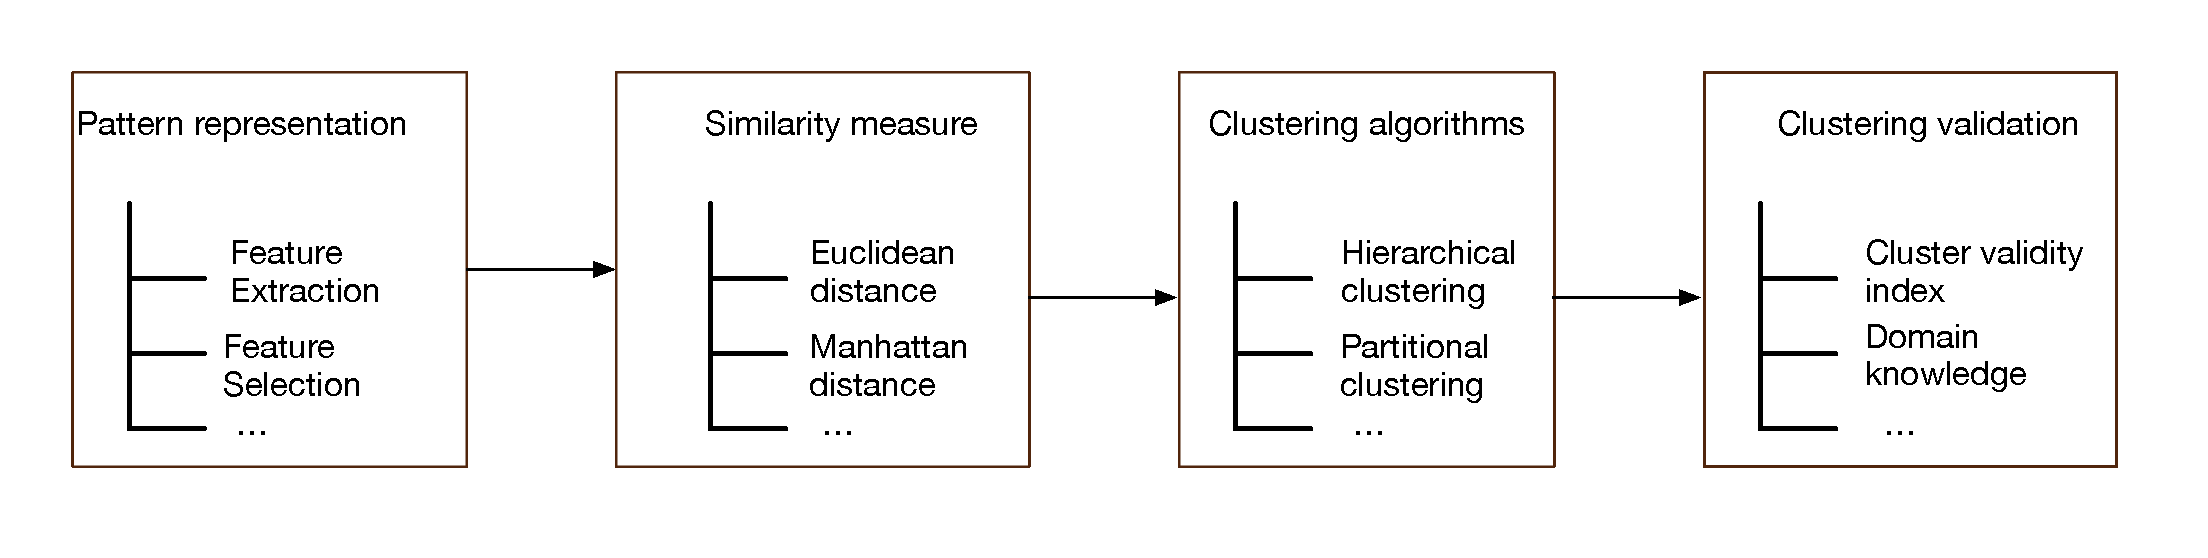
\includegraphics[scale=.32]{clustering}
%
% If no graphics program available, insert a blank space i.e. use
%\picplace{5cm}{2cm} % Give the correct figure height and width in cm
%
\caption{An overview of the basic steps constituting a clustering process \citep{clifford2006advanced}.}
\label{fig:2}       % Give a unique label
\end{figure}

In addition to the supervised learning methods, as the development in the past decades, unsupervised learning-based approaches became crucial in exploratory visualisation-driven ECG analysis, which are useful for the detection of relevant trends, patterns, and outliers \citep[e.g.][]{silipo1996supervised, lagerholm2000clustering}. 
The most widely used methods for unsupervised learning in the recent research focused on the clustering-based techniques. Clustering based methods learn the relevant similarity relationships of patterns which generate a collections of clusters \citep{bezdek1998some}. The clusters can be referred to a group of data vectors and then the similarities were calculated for the determination of class labels. Recently with the developing in neural networks techniques, the deep learning based methods would be introduced in this chapter, as the clustering methods had been described in the recent literatures \citep[e.g.][]{yeh2012analyzing, rodriguez2012unsupervised}.







%%%%%%%%%%%%%%%%%%%%%%%%%%%%%%%%%%%%%%%%%%%%%%%%%%%%%%%%%%%%%%%%%%%%%%%%%%%%%%%%%%%%%%%%% Deep Sparse Autoencoder

\section{Deep Learning in ECG Classification: A Preliminary Study Based on Deep Sparse Autoencoder}
Deep learning methods attempt to learn feature hierarchies as higher-level features are formed by the composition of lower-level features. The electrocardiography interpretation has been judged by the medical professionals, which was based on the abstractions of the perceptible features. In this model we consider the higher-level abstractions as the perceptible features, with whose composition the medical professionals can make arrhythmia judgement. The deep architecture automatic learning method is especially important for high-level abstractions, which human often do not know how to specify explicitly in terms of raw sensory input \citep{erhan}. As \citep{collobert} discussed, deep learning methods are bused on learning internal representations of data, another important advantage they offer is the ability to naturally leverage: (a) unsupervised data and (b) data from similar tasks to boost performance on large and challenging problems that routinely suffer from a poverty of labelled data. In the electrocardiography classification problem, we got plenty of unsupervised data, and the labelled data was limited as well, so it is a spontaneously idea to adapt deep learning method in this classification problem. 

\subsection{Deep Neural Networks}
The artificial neural network had been widely used in different applications, the basic 3-layer model (with only one hidden layer) is a fairly shallow network which means only shallow features can be learned via the structure. Deep neural networks were the structures in which we have multiple hidden layers, with which we can compute much more complex features from the input. Each hidden layer computes a non-linear transformation of the previous layer, a deep network can have significantly greater representational power (i.e., can learn significantly more complex functions) than a shallow one. A typical deep neural network structure as in Figure 3 makes no different from the normal multi layer neural network.

% For figures use
%
\begin{figure}[t]
\sidecaption
% Use the relevant command for your figure-insertion program
% to insert the figure file.
% For example, with the graphicx style use
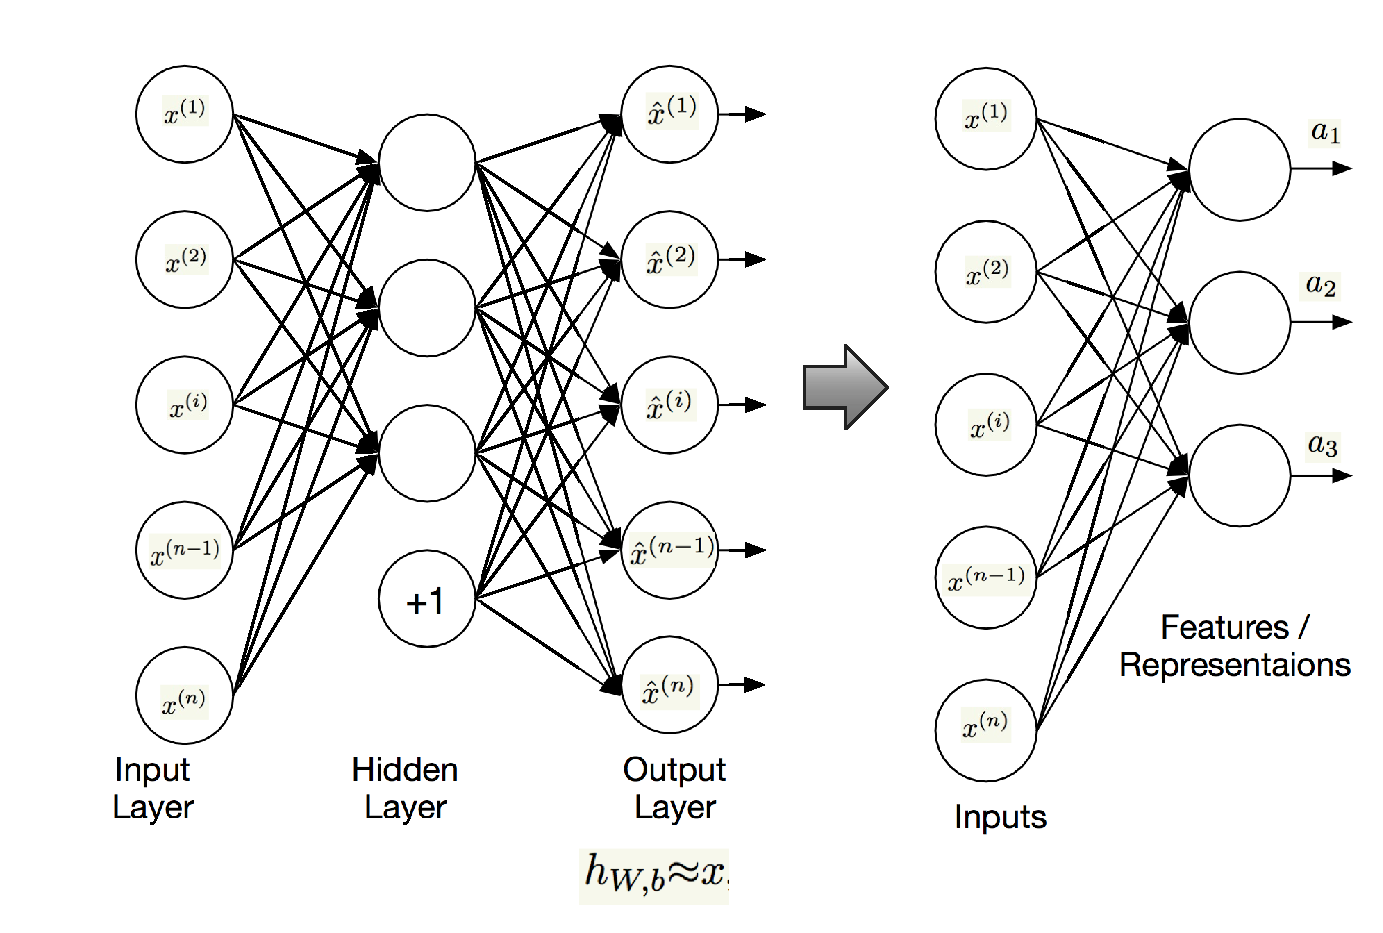
\includegraphics[scale=.5]{nnstructure}
%
% If no graphics program available, insert a blank space i.e. use
%\picplace{5cm}{2cm} % Give the correct figure height and width in cm
%
\caption{A typical neural network structure.}
\label{fig:3}       % Give a unique label
\end{figure}



\subsection{Autoencoders and Sparsity}
An autoencoder is trained to encode the input $x$ into some representation $c(x)$ so that the inputs can be reconstructed from that representation. High-dimensional data can be converted to low-dimensional codes by training a multilayer neural network with a small central layer to reconstruct high-dimensional input vectors and such "autoencoder" networks works better than principal components analysis as a tool to reduce the dimensionality of data \citep{hinton2006reducing}. Principal Component Analysis (PCA) is a linear reduction technique that seeks projection of the data into the directions of highest variability \citep{duda2012pattern}, while autoencoders do the same task in a different way with a wider scope (PCA is method that assumes linear systems where as autoencoders do not). Since in the neural network the hidden layer is nonlinear, the autoencoder behaves differently from PCA, which has the ability to capture multi-modal aspects of the input distribution (the representation of the input). The related literature experiments reported in \citep{bengio2007greedy} suggest that in practice, when trained with stochastic gradient descent, nonlinear autoencoders with more hidden units than inputs (called overcomplete) yield useful representations (in the sense of classification error measured on a network taking this representation in input). A farther defence of autoencoder can be accessed from \citep{bengio2009learning}. As the theory illustrated, the electrocardiography signal representations can be learned via the autoencoder structure and learning algorithms.

The structures and learning algorithms used were illustrated in lots of literatures \citep{duda2012pattern, bishop2006pattern}. Here we impose a sparsity constraint on the hidden units to guarantee the representations expression ability. So for the neuron in the neuron network would be "active" if its output value is close to 1, or as being "inactive" if its output value is close to 0 due to the adopted sigmoid activation function. Here $a_j^{(2)}(x)$ denote the activation of hidden unit j in the autoencoder with the given input of x. Fatherly, let 

\begin{equation}
\hat{\rho}_j = \frac{1}{m} \sum_{i=1}^m [{a_j^{(2)}}{(x^{(i)})}]
\end{equation}

\noindent be the average activation of hidden unit $j$ (averaged over the training set). Approximately enforce the constraint:

\begin{equation}
\hat{\rho}_j = \rho
\end{equation}

where $\rho$ is a sparsity parameter, typically a small value close to zero (such as $\rho = 0.05$), which means the average activation of each hidden neuron $j$ to be close to zero (0.05 for instance). 

The overall cost function of neural network is denoted by $J(W,b)$ which was defined by:

\begin{equation}
\begin{split}
J(W,b) = [\frac{1}{m}\sum_{i=1}^m(\frac{1}{2}{\|{h_{W,b}(x^{(i)})} - y^{(i)}\|}^2)] 
+ \frac{\lambda}{2}\sum_{l=1}^{n_l-1} \sum_{i=1}^{s_l} \sum_{j=1}^{s_l+1}{W_{ji}^{(l)}}^2
\end{split}
\end{equation}

\noindent as the first term in the definition of $J(W,b)$ is an average sum-of-squares error term. The second term is a regularization term that tends to decrease the magnitude of the weights, and helps prevent overfitting. The definition of $\lambda$, $s$, $l$ etc. would be explained in detail in the appendix part. To satisfy the constraint of sparsity, an extra penalty term to the optimisation objective that penalised $\hat{\rho}_j $ deviating significantly from $\rho$. The Kullback-Leibler (KL) divergence:

\begin{equation}
 \sum_{j=1}^{s_2}KL(\rho||\hat{\rho}) =  \sum_{j=1}^{s_2}\rho \text{log}{\frac{\rho}{\hat{\rho}_j}}+(1-\rho)\text{log}\frac{1-\rho}{1-\hat{{\rho}_j}}
\end{equation}

\noindent is chosen as the  penalty term. KL-divergence is a standard function for measuring how different two different distributions are. So in the autoencoder neural network training, the cost function of $J_{sparse}(W,b)$ was defined as:

\begin{equation}
J_{sparse}(W,b) = J(W,b) + \beta \sum_{j=1}^{s_2}KL(\rho||\hat{\rho_j})
\end{equation}
\noindent $\beta$ denotes the weight of the sparsity penalty term.
The above theories were cited from the recent research literatures \citep[e.g.][]{zou2012deep} and open source \citep{ufldl} on the topic of deep learning.


\subsection{Representation Learning}


% For figures use
%
\begin{figure}[]
\sidecaption
% Use the relevant command for your figure-insertion program
% to insert the figure file.
% For example, with the graphicx style use
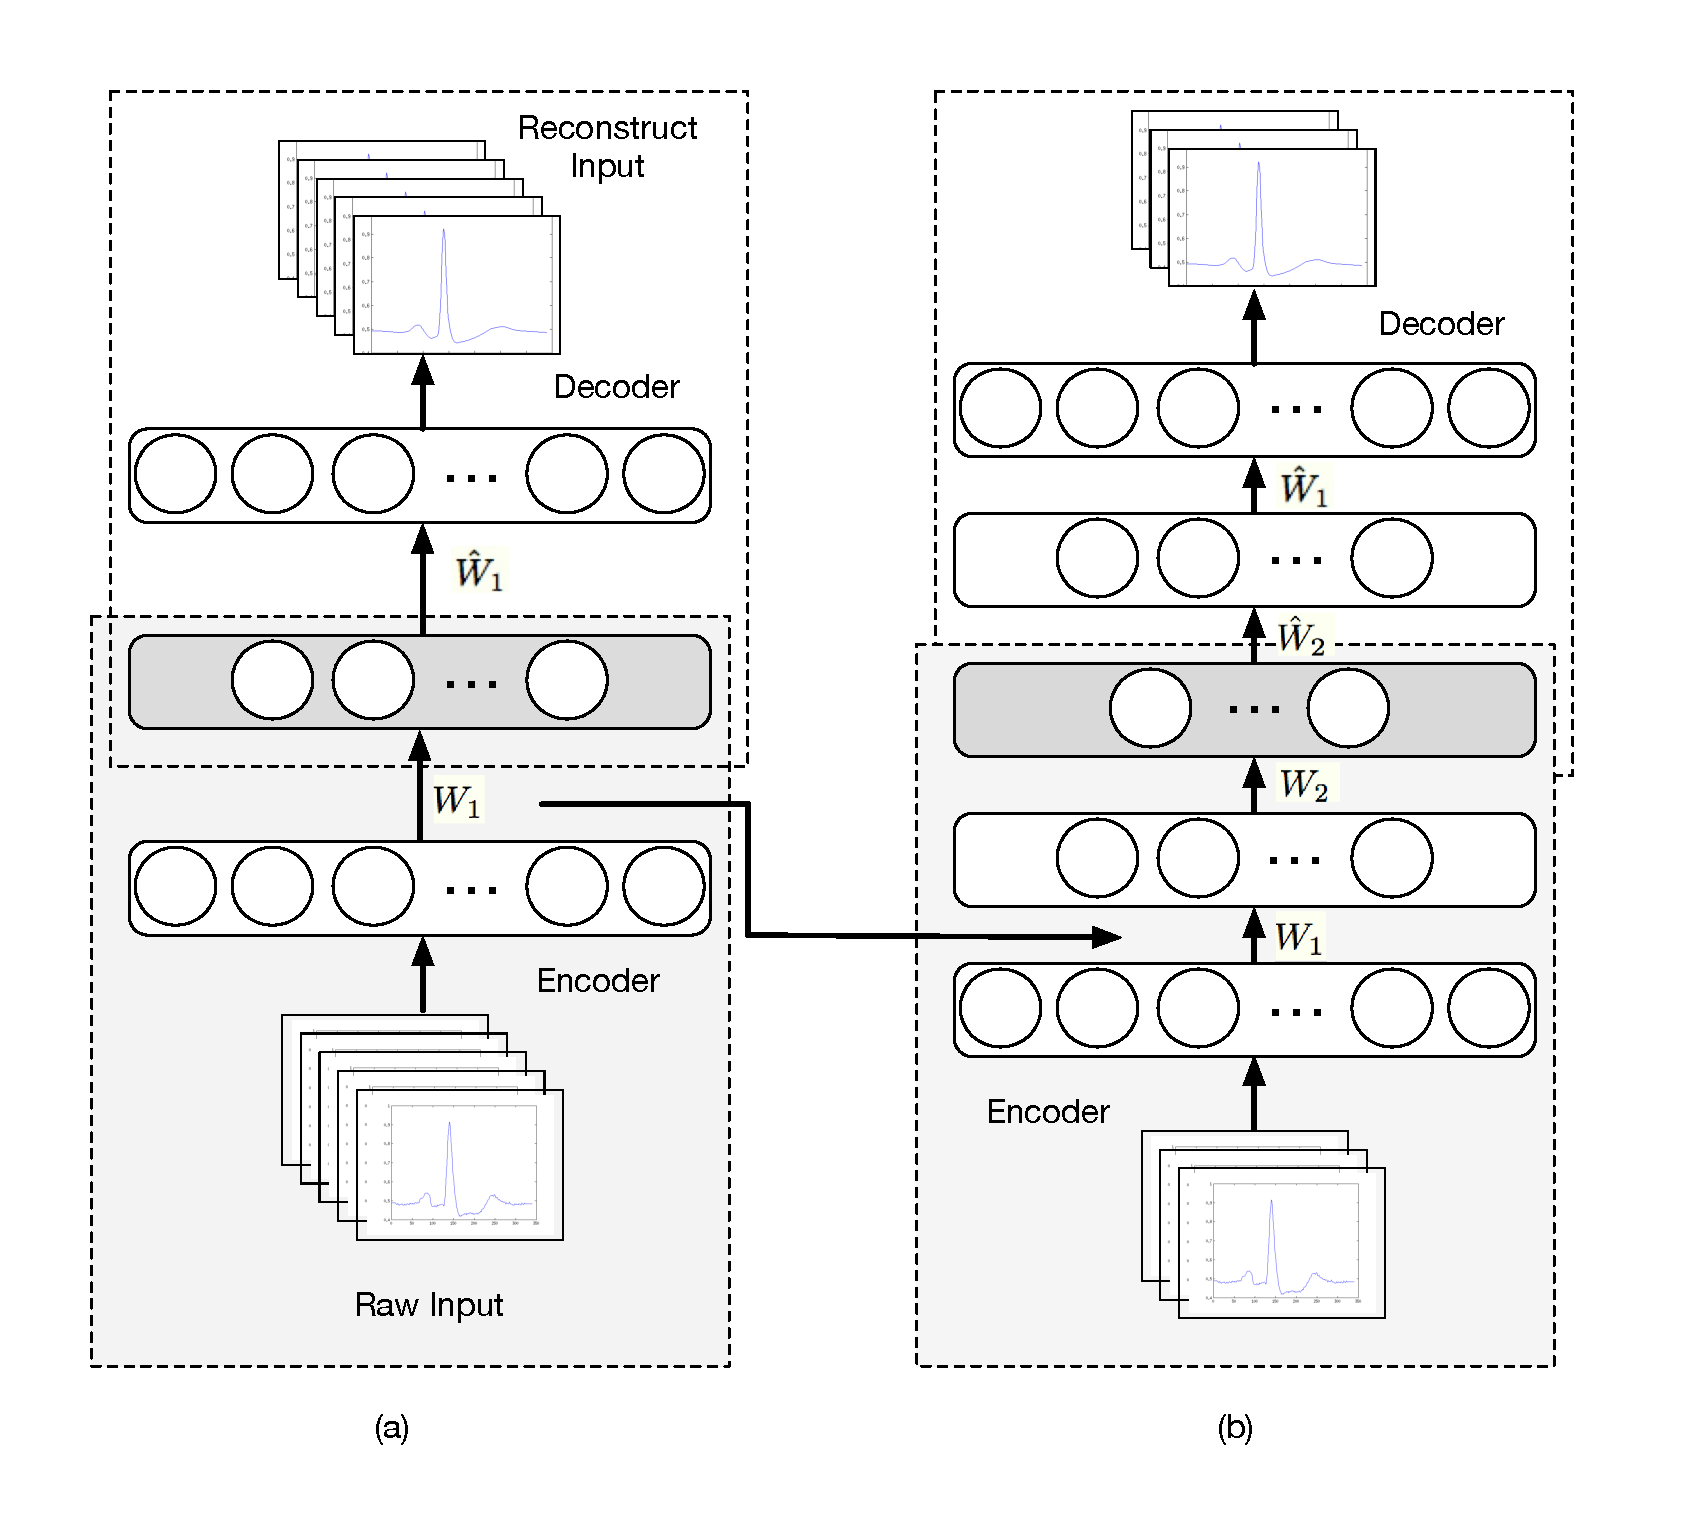
\includegraphics[scale=.4]{autoencoder}
%
% If no graphics program available, insert a blank space i.e. use
%\picplace{5cm}{2cm} % Give the correct figure height and width in cm
%
\caption{A typical autoencoder neural network structure training process.}
\label{fig:4}       % Give a unique label
\end{figure}


The autoencoder base on neuro network had been used to learn representations (features) from unlabelled data. Autoencoders have been used as building blocks to build and initialize a deep multi-layer neural network. The training procedures are illustrated in Figure \ref{fig:4} \citep{bengio2009learning}:
\begin{enumerate}
\item Train the first layer as an autoencoder to minimise some form for reconstruction error of the raw input. This is unsupervised.
\item The hidden units' outputs of the autoencoder are now used as input for another layer, also trained to be an autoencoder. Here unlabelled representations were used as well.
\item Iterates as in 2) to initialize the desired number of additional layers.
\item Take the last hidden layer output as input to a supervised layer and initialize its parameters (either randomly or by supervised training, keeping the rest of the network fixed).
\item Fine tune all the parameters of this deep architecture with respect to the supervised criterion. Alternately, unfold all the autoencoders into a very deep autoencoder and fine-tune the global reconstruction error.
\end{enumerate}
The greedy layer-wise approach for pretraining a deep network works by training each layer in turn as explained in step 2). Assume $a^{(n)}$ as the deepest activation of the autoencoder network, then $a^{(n)}$ is a higher level representation than any lower layers, which contains what we interested in. Then the higher level representations (the corresponding features in the traditional artificial selected features) can be used as the classifier input.


\subsection{Fine-tuning and Classifier}
For the training method of stacked autoencoders, when the parameters of one layer are being trained, parameters in other layer are kept fixed. In order to achieve better result, fine-tuning using backpropagation can be used to improve the model performance by tuning the parameters of all layers are changed at the same time after the layer-wise train phase. After the fine-tuning process the optimised network structure would learn a good representation of the inputs, which can be used as the features similar to the traditional methods. The cardiac arrhythmia classification problem is a multi-class classification problems where the class label $y$ may take more than two possible values.So the softmax regression is selected as the supervised learning algorithm which would be adapted as the classifier in conduction with the deep network.

Softmax regression model was generalized  from the logistic regression. Similar to the logistic regression, the training set

\begin{equation}
\{(x^{(1)},y^{(1)}), (x^{(2)},y^{(2)}), \ldots, (x^{(m)},y^{(m)}) \}
\end{equation}

\noindent of m labelled examples, the input features are $x^{(i)} \in \Re^{(n+1)}$ (with $x_0$ corresponding to there intercept term). The labels are denoted by 

\begin{equation}
y^{(i)} \in \{1,2,3,\ldots,k\}
\end{equation}
\noindent which means $k$ classes.
Given a test input $x$, the hypothesis to estimate the probability that $p(y=j|x)$ for each value of $j=1,\ldots,k$. I.e., the probabilities of the class labels taking on the $k$ different possible values are estimated. 

\begin{equation}
h_{\theta}(x^{(i)}) = 
\left[
      \begin{array}{cccccc}
        p(y^{(i)}=1|x^{(i)};\theta) \\
        p(y^{(i)}=2|x^{(i)};\theta) \\
        \vdots \\
        p(y^{(i)}=k|x^{(i)};\theta)
      \end{array}
    \right]
\end{equation}
\begin{equation}
= \frac{1}{\sum_{j=1}^ke^{\theta_j^Tx^{(i)}}}
\left[
      \begin{array}{cccccc}
        e^{\theta_1^Tx^{(i)}}\\
        e^{\theta_2^Tx^{(i)}}\\
        \vdots \\
        e^{\theta_k^Tx^{(i)}}
      \end{array}
    \right]
\end{equation}
\noindent in which $\theta_1,\theta_2,\ldots,\theta_k \in \Re^{(n+1)}$ are parameters of the model. The term $\frac{1}{\sum_{j=1}^ke^{\theta_j^Tx^{(i)}}}$ was normalizes the distribution, so that it sums to one.

The cost function adopted for softmax regression is:
\begin{equation}
J(\theta) = -\frac{1}{m}[\sum_{i=1}^m\sum_{j=1}^k1\{y^{(i)}=j\}\text{log}{\frac{e^{\theta_j^Tx^{(i)}}}{\sum_{l=1}^ke^{\theta_l^Tx^{(i)}}}}]
\end{equation}
where $1\{\cdot\}$ is the indicator function.
There is no known closed-form way to solve for the minimum of $J(\theta)$, and an iterative optimisation algorithm synch as gradient descent of L-BFGS could be used for the minimal value (some other iterative optimisation algorithms were mentioned in \citep{ngiam2011optimization}).
So the cost function and iteration equations would be:

\begin{equation}
\begin{split}
J(\theta) = -\frac{1}{m}[\sum_{i=1}^m\sum_{j=1}^k1\{y^{(i)}=j\}\text{log}{\frac{e^{\theta_j^Tx^{(i)}}}{\sum_{l=1}^ke^{\theta_l^Tx^{(i)}}}}] 
+ \frac{\lambda}{2} \sum_{i=1}^k \sum_{j=0}^n \theta_{jk}^2 (\lambda>0)
\end{split}
\end{equation}
and
\begin{equation}
\begin{split}
\bigtriangledown_{\theta_j}J(\theta) = -\frac{1}{m}\sum_{i=1}^m[x^{(i)}(1\{y^{(i)}=j\}-p(y^{(i)}=j|x^{(i)};\theta))] 
+ \lambda\theta_j  (\lambda>0)
\end{split}
\end{equation}
By minimizing $J(\theta)$ with respect to $\theta$, the softmax regression classifier would work properly for the classification task.

\subsection{Experiments and Results}
\subsubsection{Datasets Preparation}
As illustrated in the above section, the preprocessing and segmentation had been described. In the preprocessing stage, filtering algorithms were adapted to remove the artefact signals from the ECG signal. The signals include baseline wander, power line interference, and high-frequency noise. The segmentation method was based on the program of Laguna et al.\footnote{``ecgpuwave", check the website of Physionet} was adapted, which also had been validated by other related work \citep{de2004automatic}.
The experiment was based on three datasets:

\begin{enumerate}
\item Ambulatory electrocardiography database were used in this study, which includes recordings of 100 subjects with arrhythmia along with normal sinus rhythm. The database contains 100 recordings, each containing a $3-lead$ $24-hour$ long electrocardiography which were bandpass filtered at $0.1-100Hz$ and sampled at $128Hz$. In this study, only the lead I data were adapted after preprocessing in the classification task. The reference average heart beats for each sample has 97,855 beats for the $24-hour$ long recording, and the reference arrhythmia average is 1,810 beats which were estimated by a commercial software (this statistics aim to indicate the existence for arrhythmia samples, which should not be consider as a experiment preset).

\item The MIT-BIH Arrhythmia Database \citep{PhysioNet} contains 48 half- hour recordings each containing two $30min$ ECG lead signals (lead A and lead B), sampled at 360Hz. As well only the lead I data were used in the proposed method. In agreement with the AAMI recommended practice, the four recordings with paced beats were removed from the analysis.Five records randomly selected were used to verify the real time application. The remaining recordings were divided into two datasets, with small part of which were used as the training set of the fine-tuning process (details would be described in the following part).

\item The MIT-BIT Long-term Database is also used in this study for training and verification, which contains 7 long-term ECG recordings (14 to 22 hours each), with manually reviewed beat annotations and sampled at $128Hz$. Similarly, the 7 recordings were divided into two datasets, with part used as the fine- tuning training set. 

\end{enumerate}


\begin{table}
\caption{Samples after Segementation}
\label{tab:1}       % Give a unique label
%
% Follow this input for your own table layout
%
\begin{tabular}{p{5cm}p{3.2cm}p{3.1cm}}
\hline\noalign{\smallskip}
Ambulatory ECG Database (AECG) & MITBIH-AR & MITBIH-LT   \\
\noalign{\smallskip}\svhline\noalign{\smallskip}
9,785,500 & 100,687  & 667,343 \\
\noalign{\smallskip}\hline\noalign{\smallskip}
\end{tabular}
\end{table}

After the segmentation for the ambulatory ECG database, three batches of heartbeat samples listed in Table \ref{tab:1} were acquired for the classification task. 



\begin{table}
\caption{Samples Dataset Settings}
\label{tab:2}       % Give a unique label
%
% Follow this input for your own table layout
%
\begin{tabular}{p{2.9cm}p{2.8cm}p{2.8cm}p{2.8cm}}
\hline\noalign{\smallskip}
Dataset & DS1 & DS2 & DS3   \\
\noalign{\smallskip}\svhline\noalign{\smallskip}
Useage & Pre-training & Fine-tuning & Test   \\
Source(samples) & AECG (9,785,500)  &   &    \\
  & AR (50,193)   & AR (33,663) & AR (16,831) \\
  & LT (587,347)  & LT (50,000) & LT (30,000) \\
\noalign{\smallskip}\hline\noalign{\smallskip}
Total & 10,423,040 & 83,633 & 46,831 \\
\noalign{\smallskip}\hline\noalign{\smallskip}
\end{tabular}
\end{table}


As for the pretraining, fine-tuning for our proposed task and comparison, we divided all the samples into three groups: the pretraining group as DS1, the fine-tuning group as DS2 and test group as DS3 (illustrated in Table \ref{tab:2}). Samples are chosen randomly from the original AR and LT database, the details of the sample class would be described in the experiment result analysis.

\subsubsection{Classification Workflow}
The stack autoencoder use multilayer “encoder” network to transform high dimensional data into low dimensional code, similarly a “decoder” network can be adopted to recover from the code, which we previously described. For the one-hidden-layer autoencoder input layer and hidden layer, the output was set equal to the input, starting with random weights in the one-hidden layer neural networks, they can be trained together by minimizing the discrepancy between the original input data and the reconstruction. The gradients were obtained by using chain rule of backpropagate error derivatives, the decoder means the raw input can be reconstructed by the learned feature with the trained weight. With large initial weights, autoencoders typically find poor local minima; with small initial weights, the gradients in the early layers are tiny, making it infeasible to train autoencoders with many hidden layers. After learning the feature and network weight in the first layer, we can add hidden layer one by one to get deeper representations, as well the learned weight can be used to reconstruct the input. When training the weight of layer 2, we take the weight in layer 1 fixed replace random initialize because the learned weights are close to a good solution, which means training the parameters of each layer individually while freezing parameters for the remainder of the model. In the experiment, we adopted 2-hidden-layer, 3-hidden- layer, 4-hidden-layer stacked autoencoder for the test and verification.

Fine tuning is a strategy that widely used in deep learning, which can be used to greatly improve the performance of a stacked autoencoder. After pretraining multiple layers of feature detectors, the model is “unfold” to produce encoder and decoder networks that initially use the same weights. The weights learned can be used for classification implementation after adding one classifier after the feature layer. In this study, a softmax classifier was added. The parameters learned in the autoencoder pretraining were used in the fine-tuning initialization, and the weights $W$ and biases b of softmax classifier (the last layer of the network) were initialized randomly. The training set of DS2 were used in the supervised learning pretraining while the backpropagation algorithm as usual of multi-layer perceptrons to minimize the output prediction error has been adopted.

\subsubsection{Classifier Performance Assessment}
After the pretraining and fine-tuning process, the deep network parameters were acquired. Then we use the parameters and the test data set DS3 to predict the class of samples. It is necessary to mention that in DS2 and DS3, the labelled data used in pretraining and fine-tuning were divided randomly, which satisfy the requirement of Holdout cross-validation scheme so that the test results were meaningful for the classification task performance improvement.

The following statistical parameters of test performance were used in the study:
\begin{enumerate}
\item Specificity: number of correctly classified normal beats over total number of normal beats.
\item  Sensitivity: number of correctly classified abnormal beats over total number of the given abnormal beats.
\item Overall classification accuracy: number of correctly classified beats over number of total beat.
\end{enumerate}

\subsubsection{Results}



\begin{table}
\caption{Test Result for 2-Hidden-Layer Autoencoder Network}
\label{tab:3}       % Give a unique label
%
% Follow this input for your own table layout
%
\begin{tabular}{p{1.5cm}p{1.6cm}p{1.5cm}p{1.4cm}p{1.5cm}p{1cm}p{1cm}p{1.1cm}}
\hline\noalign{\smallskip}
    \multicolumn{4}{r}{Algorithm classified label}\\
    \noalign{\smallskip}\hline\noalign{\smallskip}
    &   & N      & S    & V     & F   & Q   & T\\
\noalign{\smallskip}\svhline\noalign{\smallskip}
 Reference  & N & 41,965 & 39   &  45   & 13  &  6  &  42,068 \\
	label   & S &  91    & 398  &  6    & 2   & 0   &  497\\
			& V &  63    & 3    & 3,940 & 5   & 4   &  4,015\\
			& F &  23    & 0    & 13    & 212 & 0   &  248\\
			& Q &  2     & 1    & 0      & 1   & 0   &  3\\
\noalign{\smallskip}\hline\noalign{\smallskip}
\end{tabular}

$^a$ The test accuracy is about $99.33\%$
\end{table}

As previously mentioned, we adopted three different layer strategies for the classification task. In the 2-hidden-layer autoencoder network, we got a accuracy of $99.33\%$. For the N class the specificity is $99.76\%$, the sensitivity of S class is $80.08\%$, the sensitivity of V class is $98.13\%$, the sensitivity of F class is $85.48\%$ as illustrated in Table \ref{tab:3}. 


\begin{table}
\caption{Test Results for 3-Hidden-Layer Autoencoder Network}
\label{tab:4}       % Give a unique label
%
% Follow this input for your own table layout
%
\begin{tabular}{p{1.5cm}p{1.6cm}p{1.5cm}p{1.4cm}p{1.5cm}p{1cm}p{1.1cm}p{1.1cm}}
\hline\noalign{\smallskip}
    \multicolumn{4}{r}{Algorithm classified label}\\
    \noalign{\smallskip}\hline\noalign{\smallskip}
    &   & N      & S    & V     & F   & Q   & T\\
\noalign{\smallskip}\svhline\noalign{\smallskip}
 Reference  & N & 41,721 &  66  &  66   & 19  &  0 &  41,872 \\
	label   & S &  120   & 405  &  13   & 1   & 0  &  539\\
			& V &  74    & 10   & 4,073 & 17  & 0  &  4,174\\
			& F &  27    & 2    & 19    & 196 & 0  &  244\\
			& Q &  2     & 0    & 0     & 1   & 0  &  2\\
\noalign{\smallskip}\hline\noalign{\smallskip}
\end{tabular}
$^a$ The test accuracy is about $99.07\%$
\end{table}

In the 3-hidden-layer autoencoder network, we got a accuracy of $99.07\%$. For the N class the specificity is $99.64\%$, the sensitivity of S class is $75.14\%$, the sensitivity of V class is $97.58\%$, the sensitivity of F class is $80.33\%$ as illustrated in Table \ref{tab:4}.

\begin{table}
\caption{Test Results for 4-Hidden-Layer Autoencoder Network}
\label{tab:5}       % Give a unique label
%
% Follow this input for your own table layout
%
\begin{tabular}{p{1.5cm}p{1.6cm}p{1.5cm}p{1.4cm}p{1.5cm}p{1cm}p{1.1cm}p{1.1cm}}
\hline\noalign{\smallskip}
     \multicolumn{4}{r}{Algorithm classified label}\\
    \noalign{\smallskip}\hline\noalign{\smallskip}
    &   & N      & S    & V     & F   & Q   & T\\
\noalign{\smallskip}\svhline\noalign{\smallskip}
Reference & N & 41,778 &  38  &  48   & 17  & 5  &  41,886 \\
	label  & S &  93    & 460  &   3   & 1   & 2  &  559\\
		   & V &  52    & 1    & 4,067 & 11  & 6  &  4,137\\
		   & F &  15    & 0    & 13    & 214 & 2  &  244\\
		   & Q &  1     & 0    & 1     & 1   & 1  &  5\\
\noalign{\smallskip}\hline\noalign{\smallskip}

\end{tabular}

$^a$ The test accuracy is about $99.34\%$
\end{table}

In the 4-hidden-layer autoencoder network, we got a accuracy of $99.34\%$. For the N class the specificity is $99.74\%$, the sensitivity of S class is $82.29\%$, the sensitivity of V class is $98.31\%$, the sensitivity of F class is $87.71\%$ as illustrated in Table \ref{tab:5}. 


\subsubsection{Comparison with Other Work}
Different kinds of performance assessment criteria had been adopted in the ECG arrhythmia classification problem. In the comparison part, we adopt several ordinary indicators for the performance assessment, which brought in the above sections. The accuracies, N-class specificities (N-spe), S-class sensitivities (S-sen), V-class sensitivities (V-sen) and the F-class sensitivities(F-sen) in Table \ref{tab:6} are presented for the comparison. The percentages are calculated from the literatures' test results, in which some of the classes are ignored like \citep{melgan}, we use a $*$ symbol to represent the result are not available. 
In Table \ref{tab:6}, we use the highest value (2 to 4 hidden layers based structures) for the verification which illustrated in ``proposed" line.




\begin{table}
\caption{Comparisons with Other Work Using Deep Autoencoder}
\label{tab:6}       % Give a unique label
%
% Follow this input for your own table layout
%
\begin{tabular}{p{2.6cm}p{1.7cm}p{1.7cm}p{1.7cm}p{1.7cm}p{1.6cm}}
\hline\noalign{\smallskip}
 Approaches     &  Accuracy & N-spe & S-sen & V-sen & F-sen  \\
\noalign{\smallskip}\svhline\noalign{\smallskip}
Proposed             &  \textbf{99.34\%}  & \textbf{99.76\%} &  82.29\% & \textbf{98.31\%} & 87.71\% \\
 \citet{mar2011optimization}        &  84.63\%  & 84.85\% & 82.90\%  & 86.72\% & 51.55\% \\
 \citet{chaza}   &  86.19 \% & 86.86\% & \textbf{83.83\%}  & 77.74\% & \textbf{89.43\%} \\
 \citet{melgan} &   90.52\%  & 89.12\% & *$^a$    & 89.97\% & * \\
  \citet{jiang2007block}   &  94.51\%  & 98.73\% & 50.59\%  & 86.61\% & 35.78\% \\
\noalign{\smallskip}\hline\noalign{\smallskip}
\end{tabular}

$^a$ * means the results were not available.

$^b$ The listed percentages are based on the previous described rules.
\end{table}

Through the comparisons in Table \ref{tab:6}, we can see that the proposed method offers better accuracy of classification problem. Since accuracy in lots of the literatures are good enough, the verification parameter depends on mainly on the normal class detection, but on contrary with these methods, this approach provided better performance in other kind of arrhythmia waveforms classes. Especially in the ventricular ectopic beat sensitivity, a quite large improvement had been made by the proposed method.



%%%%%%%%%%%%%%%%%%%%%%%%%%%%%%%%%%%%%%%%%%%%%%%%%%%%%%%%%%%%%%%%%%%%%%%%%%%%%%%%%%%%%%%%%Deep Belief Network

\section{Deep Learning in ECG Classification: A Two-lead ECG Classification Based on Deep Belief Network}
A restricted Boltzmann machine learning algorithm were proposed in the two-lead heart beat classification problem. A restricted Boltzmann machine (RBM) is a generative stochastic artificial neural network that can learn a probability distribution over its set of inputs \citep{fischer2012introduction}. In this part a deep belief network was constructed and the RBM based algorithm was used in the classification problem. 

\subsection{The Deep Belief Network and Classifier}

\subsubsection{The Restricted Boltzmann Machine}
The restricted Boltzmann Machine is a stochastic neural network with strong unsupervised learning ability. In the RBM network structure, each visible unit is connected to the hidden units without visible-visible or hidden-hidden connections. There were no connections between the visible and hidden layers.  The visible units were independent then the Gibbs sampling method could be used to approximate the probability distribution. It consists of one layer of visible units with input $X = (v_1, v_2,...,v_n)$, one layer of hidden units with output $Y=(h_1, h_2,...,h_m)$ and two bias units whose states were always on and a way to adjusting the value of each unit.

Boltzmann machine is based on statistical mechanics. The energy function $E(v, h)$ of an RBM was defined as:

\begin{equation}
E(v,h|\theta) = -\sum_{i=1}^n{a_iv_i}-\sum_{j=1}^m{b_ih_i}-\sum_{i=1}^n\sum_{j=1}^m{v_iW_{ij}h_j}
\end{equation}
$v$ and $h$ present the state vectors of the visible and hidden layers, $a_i$. $b_j$ and $W_{ij}$ are parameters , define $\theta = \{W_{ij}, a_i, b_j\}$. So based on the energy function, the distribution of $v$ and $h$ is:


\begin{equation}
P(v,h|\theta) = \frac{e^{-E(v,h|\theta)}}{Z(\theta)}, Z(\theta) = \sum_{v,h}^{}{e^{-E(v,h|\theta)}}
\end{equation}


The purpose of RBM is to learn the optimal $\theta$, according to the probability distribution, the maximum likelihood function is defined as:

\begin{equation}
\theta^* = arg\max\limits_{\theta}L(\theta) = arg\max\limits_{\theta}\sum_{t=1}^T{\log P(v^{(t)}|\theta)}
\end{equation}
\begin{equation}
L(\theta) = \sum_{t=1}^T\Bigg (\log\sum_{h}^{}{exp[-E(v^{(t)},h|\theta)]}-\log\sum_{v}^{}{\sum_{h}^{}{[-E(v,h|\theta)]}}\Bigg)
\end{equation}

To get the optimal $\theta^*$, stochastic gradient descent\citep[e.g.][]{leon2010large} method was used to maximum the likelihood function $L(\theta)$. The partial derivative of the parameters is shown below:

\begin{equation}
\begin{split}
&\frac{\partial\log P(v|\theta)}{\partial W_{ij}} = \langle v_i h_i \rangle_{data} -\langle v_i h_i \rangle_{model},\\
&\frac{\partial\log P(v|\theta)}{\partial a_{i}} = \langle v_i \rangle_{data} -\langle h_i \rangle_{model},\\
&\frac{\partial\log P(v|\theta)}{\partial b_{j}} = \langle h_i \rangle_{data} -\langle h_i \rangle_{model}.
\end{split}
\end{equation}
$\langle . \rangle_P$ denotes the distribution about P. $\langle . \rangle_{data}$ is easy to be calculated when the training samples were defined. $\langle . \rangle_{model}$ could not be resolved directly, but approximated by Gibbs sampling. Here we use the contrastive divergence(CD) algorithm\citep{hinton2002training} which would achieve better results by only one step of Gibbs sampling.

\subsubsection{Classifier and the Training of Multi-layer RBM}
This model generalized logistic regression\citep{peng2002intro} in classification missions which would be useful in heartbeats arrhythmia classification problems. The softmax model is a kind of supervised learning method in conjunction with the deep belief network.

Supposing $m$ samples in the training set :
\begin{equation}
\{(x^{(1)},y^{(1)}), (x^{(2)},y^{(2)}), \ldots, (x^{(m)},y^{(m)}) \}
\end{equation}
the inputs were vectors $x^{(i)}$ corresponding to the features space. The labels are denoted by $y^{(i)}$  corresponding to the arrhythmia classes of the inputs.
The cost function of softmax regression with a weight decay term was defined as:

\begin{equation}
\begin{split}
J(\theta) = -\frac{1}{m}[\sum_{i=1}^m\sum_{j=1}^k1\{y^{(i)}=j\}\text{log}{\frac{e^{\theta_j^Tx^{(i)}}}{\sum_{l=1}^ke^{\theta_l^Tx^{(i)}}}}] \\
+ \frac{\lambda}{2} \sum_{i=1}^k \sum_{j=0}^n \theta_{jk}^2 (\lambda>0)
\end{split}
\end{equation}
and the partial derivative of the parameters were:
\begin{equation}
\begin{split}
\bigtriangledown_{\theta_j}J(\theta) = -\frac{1}{m}\sum_{i=1}^m[x^{(i)}(1\{y^{(i)}=j\}-p(y^{(i)}=j|x^{(i)};\theta))] \\
+ \lambda\theta_j  (\lambda>0)
\end{split}
\end{equation}
To train an optimum classifier, an optimization gradient descent algorithm called L-BFGS was used same as what had been done in the autoencoder classification.

\begin{figure}[b]
\sidecaption
% Use the relevant command for your figure-insertion program
% to insert the figure file.
% For example, with the graphicx style use
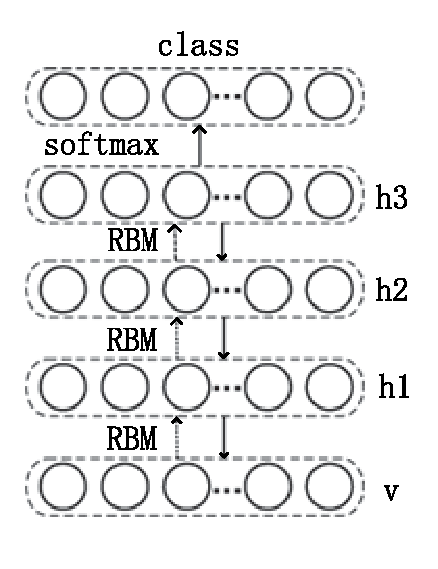
\includegraphics[scale=.3]{dbn}
%
% If no graphics program available, insert a blank space i.e. use
%\picplace{5cm}{2cm} % Give the correct figure height and width in cm
%
\caption{The RBMs are stacked to from a deep belief network(DBN). The RBM can be trained layer by layer. It is easy to construct a DBN with the trained RBMs. Also, a softmax model to fine-tune all parameters behind the last layer.}
\label{fig:5}       % Give a unique label
\end{figure}

Figure \ref{fig:5} shows that RBMs can be stacked and trained with a greedy manner to form a deep belief network(DBN) \citep{jurgen2015review, bengio2009learning}. In the last layer, a softmax classifier is connected with the DBN. DBN is the graphical model of a hierarchical architecture. The procedures were:

\begin{enumerate}
\item Train the first layer as an RBM which models the raw input $X$ as a visible layer.
\item After training the RBM, representations of the input were obtained.
\item Train the next layer as an RBM which models the transformed data as a visible layer.
\item Iterate step 2 and 3 for the desired number of layers.
\end{enumerate}

Finally the RBMs are combined to a DBN with the softmax model. Fine-tuning then was used as the supervised method to minimize the likelihood function and improve the adaptability. Here the L-BFGS algorithm\citep{liu1989limited, andrew2007scalable} was used.

\subsubsection{Combined optimization algorithm for multi-lead classifiers}
The ECG wavelet transform performs differently in different channels by the waveforms. Each heartbeat channel shows diversely due to the P,QRS-complex and T wave constituent. 
Taking those into consideration, multi-lead ECG classification is significant improved by sample voting method. So a weight optimization method is proposed in two leads ECG signal classification. 
The method can be generally used in multi-lead ECG data classification. 

For each classifier trained with distinct lead, a reliability value is denoted as the accurate rate of the classifier. let $\gamma$ represent the reliability value. Then the classifiers' reliability is defined as $\gamma_1, \gamma_2, \cdots$

Using the testing samples to assess the result. The statistical matrix:
\begin{equation}
ClassSTST = \left(
\begin{array}{cccc}
 C_{11} & C_{12} & \cdots & C_{1n}\\
 C_{21} & C_{12} & \cdots & C_{2n}\\
 \cdots & \cdots & \ddots & \cdots\\
 C_{n1} & C_{n2} & \cdots & C_{nn}
\end{array}
\right)~
\end{equation}
In the statistical matrix, there are $n$ classes and $C_{11}$ represents the class \uppercase\expandafter{\romannumeral1} which is classified as class \uppercase\expandafter{\romannumeral1}, $C_{12}$ represents class \uppercase\expandafter{\romannumeral1} is classified as \uppercase\expandafter{\romannumeral2}, etc. 
The diagonal values are the correct classification. The purpose is to increase the diagonal values, so we adopt weights of the outputs for each classifier. 
The weights of the first classifier is $W_1 = (w_{11}, w_{12}, \cdots, w_{1n})$, the second were $W_2 = (w_{21}, w_{22}, \cdots, w_{2n})$. The constraint condition is $\sum\nolimits_{i=1}^2{w_{ik}} = 1$. 

First initial the weight to a mean value. Each sample has an output vector $O = {o_1, o_2, \cdots, o_n}$, the class is decided by the maximum value. Adding the weight of the value, the output is $(o_1w_1 ,o_2w_2, \cdots, o_nw_n)$. If the label of the sample is $l$, we would like to maximize $o_1w_{11} + o_1w_{21}$ while correspondingly minimize others. Through this, the $l$ class accurate is promoted while the false negative rate is also increased. The optimization algorithm would find a balance between the two weights of all testing samples. Accordingly, the optimal function is defined as:
\begin{equation}
F(x) = \frac{1}{\sqrt{2\pi}\sigma}x\exp^{-\frac{(x-\mu)^2}{2\sigma^2}}
\end{equation}
To find the maximum value of x, the derivative of the equation is:
\begin{equation}
\begin{split}
F^{'}(x) = 0, x = \frac{\mu}{2}+\sqrt{\frac{\mu^2}{4}+\sigma^2}
\end{split}
\end{equation}
Here, $\mu$ is denoted as initial weights. On the basis of the statistical matrix , counting the difference of the correct (diffcort) and false negative (diffflneg) quantities of the two classifiers. If the difference of the difference of the correct and false negative greater than zero, $\sigma^2 = \sqrt{\frac{diffcort - diffflsneg}{totalnumber}}$, so updating the corresponding class weight of the first classifier as $w_1 = \frac{\mu}{2}+\sqrt{\frac{\mu^2}{4}+\sigma^2}$. Else, $\sigma^2 = \sqrt{\frac{diffflsneg - diffcort}{totalnumber}}$, updating the weight of the second classifier as $w_2 = \frac{\mu}{2}+\sqrt{\frac{\mu^2}{4}+\sigma^2}$. Finally normalize the weights, the optimal combined value is $\gamma_1o_1w_1 + \gamma_2o_2w_2$. Generally, every two classifiers can be used to optimize the multi-lead ECG classification.



\subsection{Experiment  and Results}
\subsubsection{Preprocessing and Segmentation}
Here we do the same process as the above sparse autoencoder network diid. The experiment data sets changed due to the new problem. The preprocessing include two main parts: the ECG data filtering and heartbeat segmentation. The filtering task is removing the artifact signal from the ECG signal, which includes the baseline wander, power line interference and high-frequency noise. The  massive unlabelled data we collected is extracted and resampled from $128Hz$ to $360Hz$. 

In heartbeat segmentation process, average samples of each beat is 277 samples. To get more information , we allow partially overlap and a window with a length of 340 data points in one beat was defined, the R peak of the wave is located at 141st point. Most annotations of the MIT-BIH arrhythmia database lied under the R-wave. For the dataset we collect, a high accurate algorithm has been explored to determine the R pick and then divide into the heartbeat segments according to the R pick.

\subsubsection{Training and Fine-tuning}
The goal of RBM learning is to maximize the product of the probabilities. The parameters of the network can be initialized by the constructor. This option is useful when an RBM is used as the building block of the deep belief network, in which case the weight matrix and the hidden layer bias is shared with the corresponding layer of the network. The active function of the nodes is sigmoid function. The data is batched to train the RBM layer by layer. A single-step contrastive divergence(CD-1) \citep{carreira2005contrastive} is used in the gradient descent procedure. After calculating the partial derivative, the weights and bias is updated.

After the learning process, the RMBs can be used to initialize a deep belief network. Standard backpropagation algorithm can be applied to fine-tune the model. That can significantly improve the performance of the DBN. The fine- turning process is a supervised learning procedure, so at the last layer, a multi-class model called softmax is connected to classify the ECG data. Then using the fine-turning method to minimize the cost function.

\subsubsection{Experiment Results}

In the experiments, we adopted multi-lead ECG signal based on the restricted Boltzmann machine for the classification task. The MIT-BIH arrhythmia database is divided into three parts. Half of the beat is added to training the RBMs, one-third is applied to fine-tune the network and the left is used to test the model. In the 3 hidden layers deep belief network, the classifier outperforms in terms of sensitivity (SPR) $99.35\%$, specificity (SPC) $95.18\%$ and accuracy rate (ACC) $98.25\%$ using the first channels. Using the second channel we get the accuracy (ACC) of $97.43\%$, sensitivity (SPR) $98.90\%$ and specificity (SPC) $93.36\%$. At convergence of the optmization process, the combining method achieves the accuracy (ACC) of $98.83\%$, sensitivity (SPR) $99.83\%$ and specificity (SPC) $96.05\%$.



\begin{table}
\caption{Test result of three hidden Layers deep belief network using the first lead}
\label{tab:7}  
\begin{tabular}{p{1cm}p{1.2cm}p{0.9cm}p{0.7cm}p{0.7cm}p{0.6cm}p{0.6cm}p{0.6cm}p{0.7cm}p{0.6cm}p{0.6cm}p{0.6cm}p{0.7cm}p{0.7cm}}
\hline\noalign{\smallskip}
\multicolumn{9}{r}{Algorithm classified label} \\
\noalign{\smallskip}\hline\noalign{\smallskip}
		 &      & N* & L* & R* & AB* & P* & FU* & NPC & APC & FL* & V* & NE*& AE*\\
\noalign{\smallskip}\svhline\noalign{\smallskip}
 		 & NORMAL & 12,289& 3   &  2   &  3   &  15  &  9    &	0   &  37 &   2   &   0  &  0  &  0 \\
	     & LBBB   &  7    & 1,369&  0  &  0   &  6   &  0    &  0   &  1  &   0   &   0  &  0  &  0 \\
		 & RBBB   &  4    &  0  & 1,179&  0   &  3   &  0    &	0   &  4  &   0   &   0  &  0  &  0 \\
		 & ABERR  &  7    &  1  &  0   &  12  &  5   &  0    &	0   &  0  &   1   &   0  &  0  &  0 \\
		 & PVC    &  18   &  2  &  0   &  2   & 1,104&  8    &	0   &  2  &   2   &   0  &  0  &  0 \\
Original & FUSION &	 19   &  0  &  0   &  1   &  6   &   97  &	0   &  0  &   0   &   0  &  2  &  0 \\
label    & NPC    &	 5    &  0  &  1   &  0   &  0   &  0    &	4   &  1  &   0   &   0  &  1  &  0 \\
		 & APC    &	 58   &  2  &  9   &  0   &  2   &  0    &	0   &  382&   0   &   0  &  2  &  0 \\
		 & FLWAV  &	 10   &  0  &  0   &  1   &  8   &  0    &	0   &  0  &   58  &   0  &  0  &  0 \\
		 & VESC   &	 2    &  0  &  0   &  0   &  1   &  0    &	0   &  0  &   0   &  24  &  0  &  0 \\
		 & NESC   &	 6    &  0  &  1   &  0   &  0   &  0    &	0   &  1  &   0   &   0  &  15 &  0 \\
		 & AESC   &	 3    &  0  &  0   &  0   &  0   &  0    &	0   &  0  &   0   &   0  &  0  &  0 \\

\noalign{\smallskip}\hline\noalign{\smallskip}
\end{tabular}
$^a$ The test accuracy of the first lead is $98.247\%$

$^b$ Use N* as NORMAL for abbreviation and the same for the rest symbols
\end{table}




\begin{table}
\caption{Test result of three hidden Layers deep belief network using the first lead}
\label{tab:8}  
\begin{tabular}{p{1cm}p{1.2cm}p{0.9cm}p{0.7cm}p{0.7cm}p{0.6cm}p{0.6cm}p{0.6cm}p{0.7cm}p{0.6cm}p{0.6cm}p{0.6cm}p{0.7cm}p{0.7cm}}
\hline\noalign{\smallskip}
\multicolumn{9}{r}{Algorithm classified label} \\
\noalign{\smallskip}\hline\noalign{\smallskip}
		 &      & N* & L* & R* & AB* & P* & FU* & NPC & APC & FL* & V* & NE*& AE*\\
\noalign{\smallskip}\svhline\noalign{\smallskip}
		 & NORMAL & 12,233& 7   &  3   &  3   &  57  &  13   &	1   &  34 &   12  &   0  &  6  &  0 \\
	     & LBBB   &  12   & 1,366&  0  &  0   &  5   &  0    &  0   &  0  &   0   &   0  &  0  &  0 \\
		 & RBBB   &  5    &  0  & 1,169&  0   &  5   &  0    &	0   &  9  &   2   &   0  &  0  &  0 \\
		 & ABERR  &  7    &  0  &  1   &  10  &  6   &  0    &	1   &  0  &   1   &   0  &  0  &  0 \\
		 & PVC    &  56   &  3  &  1   &  0   & 1,048&  15   &	0   &  4  &   11  &   0  &  0  &  0 \\
Original & FUSION &	 22   &  0  &  0   &  0   &  5   &   97  &	0   &  0  &   0   &   0  &  1  &  0 \\
label    & NPC    &	 1    &  0  &  1   &  0   &  0   &  0    &	10  &  0  &   0   &   0  &  0  &  0 \\
		 & APC    &	 60   &  4  &  8   &  0   &  11  &  2    &	0   &  368&   1   &   0  &  0  &  1 \\
		 & FLWAV  &	 7    &  0  &  0   &  0   &  8   &  0    &	0   &  1  &   61  &   0  &  0  &  0 \\
		 & VESC   &	 2    &  0  &  1   &  0   &  2   &  0    &	0   &  0  &   2   &  20  &  0  &  0 \\
		 & NESC   &	 6    &  0  &  1   &  0   &  1   &  0    &	0   &  0  &   0   &   0  &  15 &  0 \\
		 & AESC   &	 2    &  0  &  0   &  0   &  0   &  0    &	0   &  0  &   0   &   0  &  0  &  1 \\
\noalign{\smallskip}\hline\noalign{\smallskip}
\end{tabular}
$^a$ The test accuracy of the second is $97.433\%$
\end{table}




\begin{table}
\caption{Test result of three hidden Layers deep belief network using the first lead}
\label{tab:9}  
\begin{tabular}{p{1cm}p{1.2cm}p{0.9cm}p{0.7cm}p{0.7cm}p{0.6cm}p{0.6cm}p{0.6cm}p{0.7cm}p{0.6cm}p{0.6cm}p{0.6cm}p{0.7cm}p{0.7cm}}
\hline\noalign{\smallskip}
\multicolumn{9}{r}{Algorithm classified label} \\
\noalign{\smallskip}\hline\noalign{\smallskip}
		 &      & N* & L* & R* & AB* & P* & FU* & NPC & APC & FL* & V* & NE*& AE*\\
\noalign{\smallskip}\svhline\noalign{\smallskip}
	 & NORMAL & 12,348& 0   &  0   &  0   &  11  &  2    &	0   &  7  &   1   &   0  &  0  &  0 \\
	     & LBBB   &  3    & 1,377&  0  &  0   &  3   &  0    &  0   &  0  &   0   &   0  &  0  &  0 \\
		 & RBBB   &  1    &  0  & 1,182&  0   &  2   &  0    &	0   &  5  &   0   &   0  &  0  &  0 \\
		 & ABERR  &  8    &  0  &  0   &  16  &  2   &  0    &	0   &  0  &   0   &   0  &  0  &  0 \\
		 & PVC    &  16   &  0  &  0   &  0   & 1,108&  10   &	0   &  1  &   3   &   0  &  0  &  0 \\
Original & FUSION &	 22   &  0  &  0   &  0   &  4   &   99  &	0   &  0  &   0   &   0  &  0  &  0 \\
label    & NPC    &	 3    &  0  &  0   &  0   &  0   &  0    &	9   &  0  &   0   &   0  &  0  &  0 \\
		 & APC    &	 58   &  2  &  5   &  0   &  1   &  0    &	0   &  389&   0   &   0  &  2  &  0 \\
		 & FLWAV  &	 2    &  0  &  0   &  0   &  6   &  0    &	0   &  0  &   69  &   0  &  0  &  0 \\
		 & VESC   &	 3    &  0  &  0   &  0   &  1   &  0    &	0   &  0  &   0   &  23  &  0  &  0 \\
		 & NESC   &	 11   &  0  &  1   &  0   &  0   &  0    &	0   &  1  &   0   &   0  &  11 &  0 \\
		 & AESC   &	 3    &  0  &  0   &  0   &  0   &  0    &	0   &  0  &   0   &   0  &  0  &  0 \\
\noalign{\smallskip}\hline\noalign{\smallskip}
\end{tabular}
$^a$ The test accuracy of the second is $98.829\%$
\end{table}




For we collect large amount of ECG data from the hospital which contains lots of normal beats and abnormal beats, the learning method of restricted Boltzmann machine is used to learning the features from the massive data by an unsupervised way. Then the RBMs is adapted to build a deep belief network. The optimization algorithm we propose improves the accuracy with multilead ECG signal. In this comparison, we evaluate the performance on the indicators which put forward in the above sections: Sensitivity(TPR), specificity(SPC) and overall Accuracy(ACC) with the SVM, ICA, ANN methods. The $*NR$ symbol represents the result is not reported. 

\begin{table}
\caption{Comparisons with others' works}
\label{tab:10}       % Give a unique label
%
% Follow this input for your own table layout
%
\begin{tabular}{p{2.9cm}p{2.8cm}p{2.8cm}p{2.8cm}}
\hline\noalign{\smallskip}
Approaches & Accuracy(ACC) & Sensitivity(TPR)  & Specificity(SPC)  \\
\noalign{\smallskip}\svhline\noalign{\smallskip}
Proposed                        & 98.83\%  & 99.83\%    & 96.05\%\\
\citeauthor{tadejko2007}	   & 97.82\%  & 99.70\%     & 93.10\%  \\
\citeauthor{banerjee2014app} & 97.60\%   & 97.30\%    & 98.80\%    \\
\citeauthor{can2012heartbeat}                & 99.71\%   &  *NR          & *NR      \\
\citeauthor{osowski2001ecg}  & 96.06\%   & 98.10\%    & 95.53\%     \\
\noalign{\smallskip}\hline\noalign{\smallskip}
\end{tabular}
$^a$ *NR means the results were not reported

$^b$ The listed percentages are based on the assessment rules
\end{table}


The Table \ref{tab:10} shows the performance of different models that used for the heartbeat classification, the proposed method offers a high accuracy of classification. 
All the annotations in the MIT-BIH arrhythmia database is used in our study and \citet{osowski2001ecg} only selects 7 types. \citet{can2012heartbeat} get the highest accuracy but with a price of rejecting 2,054 heartbeats($2.4\%$ rejections). By comparing with others' experience, our approach provided higher performance in heartbeat classification without complex wavelet transform algorithms. 


\section*{Conclusion}
ECG annotation research had been developed for decades, the signal processing methods, feature extraction and classifier had been studied diffusely. In this paper, we first reviewed the technique roadmap for a ECG classification task, which composed most of the ECG classification research literatures. Then we make a  short summary on the classification methodology including supervised learning and unsupervised learning, which included most ECG classification methods.  Then two kinds of new methods in unsupervised learning had been proposed for ECG annotations, which improve the state-of-art in accuracy and special arrhythmia beat detection rate.

Since the deep network autoencoder structure and deep belief network with the training algorithms had been widely used in modern computing science, an intuitionistic idea is the application in the large ECG recordings. This study proposed one possibility to adopt this method in the health informatics Big Data applications. From both the one lead deep autoencoder based ECG classification system and two-lead deep brief network based classification system, we both get higher performance than the recent research in this domain, and as the evolvability of the system, the performance could be improved as the dataset grows, form which a new possibility to make use of the large amount of unlabelled ECG data from the long-term clinical monitoring and healthcare monitoring had been proposed. Since the pre-training and fine-tuning bring the systems with  the ability of self-learning, the structures could be better optimized as the training samples become larger, especially for the rare abnormalities (the S, V, F class, check Table \ref{tab:6}). In the traditional literatures the MIT or AHA datasets were used which limited the samples of the abnormalities, so there were no good sensitivities, on the contrary using the unlabelled data and the self-learning ability the system could be improved in these outlier detections.


%\section*{Appendix}
%\addcontentsline{toc}{section}{Appendix}
%
%


%%%%%%%%%%%%%%%%%%%%%%%% referenc.tex %%%%%%%%%%%%%%%%%%%%%%%%%%%%%%
% sample references
% %
% Use this file as a template for your own input.
%
%%%%%%%%%%%%%%%%%%%%%%%% Springer-Verlag %%%%%%%%%%%%%%%%%%%%%%%%%%
%
% BibTeX users please use
\bibliographystyle{spbasic}
\bibliography{reference}

\end{document}
